\chapter{Mesures préliminaires}
\par Afin de contrôler le plus finement possible les valeurs de luminance et de contraste proposées aux sujets pendant les expérimentations, il est nécessaire de mesurer avec le plus grand soin, directement sur le simulateur, toutes ces valeurs. Les mesures ont été faites dans les conditions de l'expérimentation avec un <<~chromameter CS-100~>> (Fig. \ref{fig:chromameter_cs100}).

\begin{figure}
	\centering
	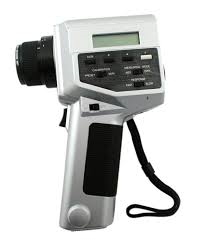
\includegraphics[scale=1]{Figures/ChromameterCS100}
	\caption{Chromameter CS100}
	\label{fig:chromameter_cs100}
\end{figure}
	
	\section{Luminance globale (luminance de fond)}
	\par La première étape est de mesurer la luminance globale du simulateur, toutes faces allumées. Dans notre expérimentation, le simulateur sert à la fois de support pour afficher les cibles visuelles à percevoir et à la fois de source principale de lumière, toutes autre lampe dans la pièce étant éteinte. Le luminance globale de l'expérimentation est donc la luminance des écrans, que l'on appellera ici <<~luminance de fond~>> pour les calculs de contraste, les cibles étant affichées directement sur une couleur uniforme sur l'écran.
	
	\par Même si il existe des manières théoriques de convertir une couleur et son code RGB associé en une luminance générée par l'écran, il est nécessaire pour nous de mesurer cette transformation. En effet, il existe un certain nombre de biais tels que l'influence des autres écrans sur l'écran mesuré, l'influence des sources mineures de lumière, la fatigue de la lampe du projecteur, la dégradation de l'écran. En mesurant la relation couleur luminance générée directement dans le simulateur, on se débarrasse de tous ces biais et on peut viser la fonction de transfert réelle.
	
	\par On effectue l'intégralité de nos mesures sur la face avant du simulateur car l'expérimentation ne se déroulera que sur cette face. Néanmoins, toutes les autres faces du simulateur sont éclairées, comme dans les conditions expérimentale, afin de prendre en compte l'influence de la luminosité des faces latérales et de la face au sol sur la luminosité de la face avant. On utilise cinq points de mesure sur la face avant (répartis à la manière d'un dé à 6 faces), chaque mesure par point étant triplée pour éviter tout effet indésirable.
	
	\par Les mesures ne sont faites que sur des nuances de gris. Pour ce faire, on affiche des couleurs dont les composantes R, G et B sont égales. Dans le simulateur, la couleur étant codée sur 8 bits, on peut afficher 256 nuances différentes: du noir le plus <<~pur~>> (Code RGB: $(0,~0,~0)$) au blanc le plus <<~pur~>> (Code RGB: $(255,~255,~255)$). Néanmoins, par soucis de praticité, on se limite à 17 nuances de gris en faisant des incréments de 16 en 16 dans le codage RGB des couleurs affichées. Par la suite, comme les trois composantes R, G et B sont toujours égales, on parlera de <<~niveau de gris~>> on se référant directement à la valeur des composantes. Par exemple, le noir sera appelé <<~gris 0~>> étant donné que c'est une nuance de gris et que ses trois composantes R, G et B sont égales à 0.
	
	\par Un extrait des résultats de mesure est disponible en Table \ref{tab:extrait_mesure_luminance_fond}, l'ensemble des mesures, détaillé par point de mesure, est disponible en annexes.
	
	\begin{table}[h]	
		\centering
		\caption{Extrait des mesures de luminance globale du simulateur en fonction de la nuance de gris affichée.}
		\label{tab:extrait_mesure_luminance_fond}
		\small
		\begin{tabular}{ccc}
			\textbf{Couleur affichée} & \textbf{Niveau de gris} & \textbf{Moyenne}\\
			Noir & 0 & $0.07~cd/m^2$\\
			Gris sombre & 80 & $3.73~cd/m^2$\\
			Gris clair & 176 & $23.22~cd/m^2$\\
			Blanc & 255 & $42.82~cd/m^2$
		\end{tabular}
	\end{table}
	
	\par On peut alors ensuite tracer le graphe représentant l'évolution de la luminance globale du simulateur en fonction du niveau de gris affiché sur toutes ses faces (Fig. \ref{fig:evolution_luminance_background}). De cette courbe, on déduit alors une régression polynomiale d'ordre 3 ($R^2 = 1$) qui nous donne la relation mathématique (Eq. \ref{eq:regression_luminance_globale}) permettant d'anticiper la luminance en fonction du niveau de gris. Cela nous permettra par la suite le choisir précisément les couleurs à afficher pour obtenir le contraste désiré. Avec $L_G$ la luminance globale du simulateur et $g$ le niveau de gris normalisé, c'est à dire variant de 0 ($= 0/255$) à 1 ($= 255/255$).
	
	\begin{equation}
		L_G(g) = 0.69 - 18.37~g + 102.08~g^2 -40.78~g^3
		\label{eq:regression_luminance_globale}
	\end{equation}
	
	\begin{figure}
		\centering
		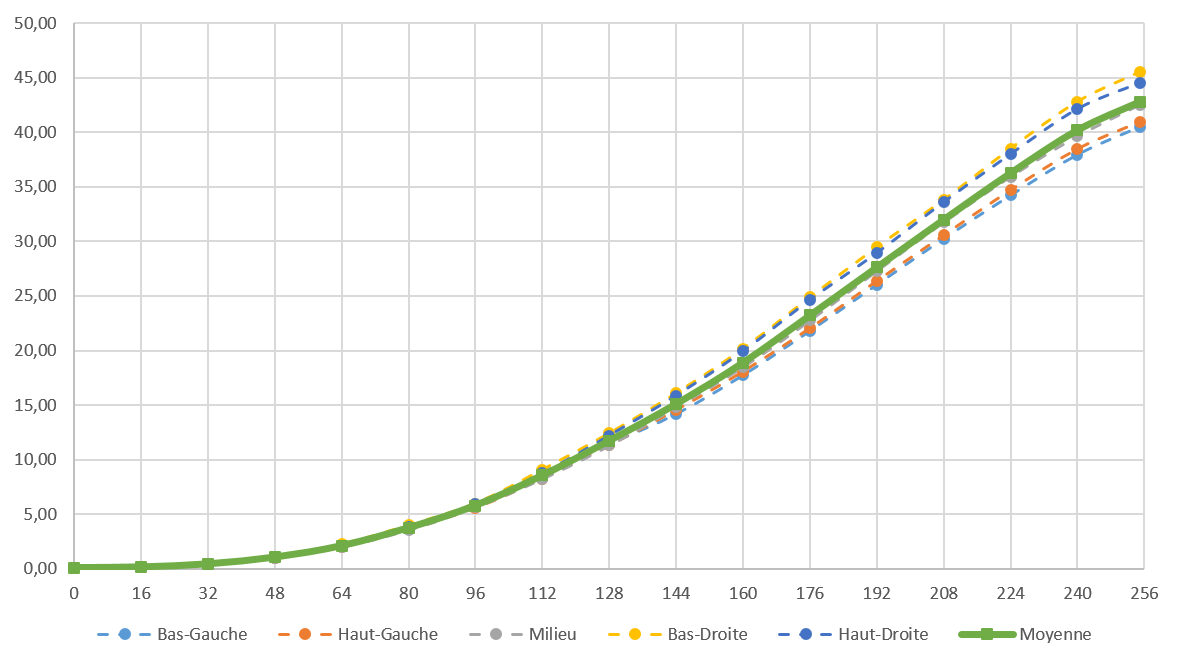
\includegraphics[scale=.75]{Figures/EvolutionLuminanceGlobale}
		\caption{Evolution de la luminance en fonction du niveau de gris sur les cinq points de mesure et leur moyenne.}
		\label{fig:evolution_luminance_background}
	\end{figure}
	
	\section{Luminance de la cible (luminance de tache)}
	\par De la même manière, on réalise ensuite une série de mesures avec, en plus de l'intégralité des faces affichant un niveau de gris uni, un petit disque d'un diamètre de 3 cm, au centre de la face avant, dans une nuance de gris différente du fond. Cette cible sera la tache visuelle à détecter pour les sujets de l'expérimentation. Il est donc nécessaire de connaitre également son évolution en luminance en fonction de son niveau de gris, le tout en fonction du niveau de gris du reste des écrans du simulateur qui vont très certainement influer.
	
	\par On limite cette fois à 6 le nombre de conditions de niveau de gris pour le reste des écrans (les 6 niveaux qui ont été retenus pour l'expérimentation) tout en gardant l'incrément de 16 par 16 pour les niveaux de gris du disque. A cause de la taille de la cible à mesurer par rapport à la surface totale des écrans, on fait l'hypothèse que celle-ci ne perturbera pas la luminance globale tandis que le niveau de gris global influera sur la luminance du disque. De même, on ne réalise qu'une seule mesure au centre du disque, triplée encore une fois.
	
	\par On présente un extrait des résultats des mesures en Table \ref{tab:extrait_mesure_luminance_target}. L'ensemble des mesures est également disponible en annexes.
	
	\begin{table}[h]	
		\centering
		\caption{Extrait des mesures de luminance du disque en fonction de sa nuance de gris et de la nuance globale affichée.}
		\label{tab:extrait_mesure_luminance_target}
		\small
		\begin{tabular}{cccc}
			\textbf{Nuance de la cible} & \textbf{Fond: 0} & \textbf{Fond: 128} & \textbf{Fond: 255}\\
			0 & $0.06~cd/m^2$ & $5.51~cd/m^2$ & $20.30~cd/m^2$\\
			64 & $1.13~cd/m^2$ & $6.55~cd/m^2$ & $21.40~cd/m^2$\\
			144 & $8.20~cd/m^2$ & $13.57~cd/m^2$ & $28.40~cd/m^2$\\
			255 & $23.37~cd/m^2$ & $28.77~cd/m^2$ & $43.40~cd/m^2$
		\end{tabular}
	\end{table}
	
	\par On s'aperçoit que l'influence du niveau de gris du reste des écrans est très grand sur la luminance de la cible au centre de l'écran principal avec par exemple une multiplication par quasiment 300 de la luminance d'un cible noire (gris 0) sur fond noir (gris 0) par rapport à une cible noire (gris 0) sur fond blanc (gris 255).
	
	\par On peut alors ensuite tracer les graphe représentant les évolutions de la luminance du disque en fonction du niveau de son niveau de gris et de celui affiché sur toutes ses faces (Fig. \ref{fig:evolution_luminance_target}). De ces courbes, on déduit les fonctions de transfert par régression polynomiale d'ordre 3 ($R^2 = 1$) (Eq. \ref{eq:regression_luminance_cible}). Avec $L_{T,p}$ la luminance du disque sur la face avant du simulateur et $g$ le niveau de gris normalisé de la cible et $p$ celui du reste des écrans.
	
	\begin{equation}
		\begin{cases}
		L_{T,0}(g) = 0.44 - 10.67~g + 56.44~g^2 - 22.37~g^3\\
		L_{T,32}(g) = 0.60 - 10.67~g + 56.33~g^2 - 22.25~g^3\\
		L_{T,80}(g) = 2.11 - 10.87~g + 59.90~g^2 - 22.64~g^3\\
		L_{T,128}(g) = 5.89 - 10.74~g + 56.29~g^2 - 22.24~g^3\\
		L_{T,176}(g) = 11.45 - 10.33~g + 54.77~g^2 - 21.11~g^3\\
		L_{T,255}(g) = 20.69 - 10.85~g + 57.24~g^2 - 23.21~g^3
		\end{cases}
		\label{eq:regression_luminance_cible}
	\end{equation}
	
	\begin{figure}
		\centering
		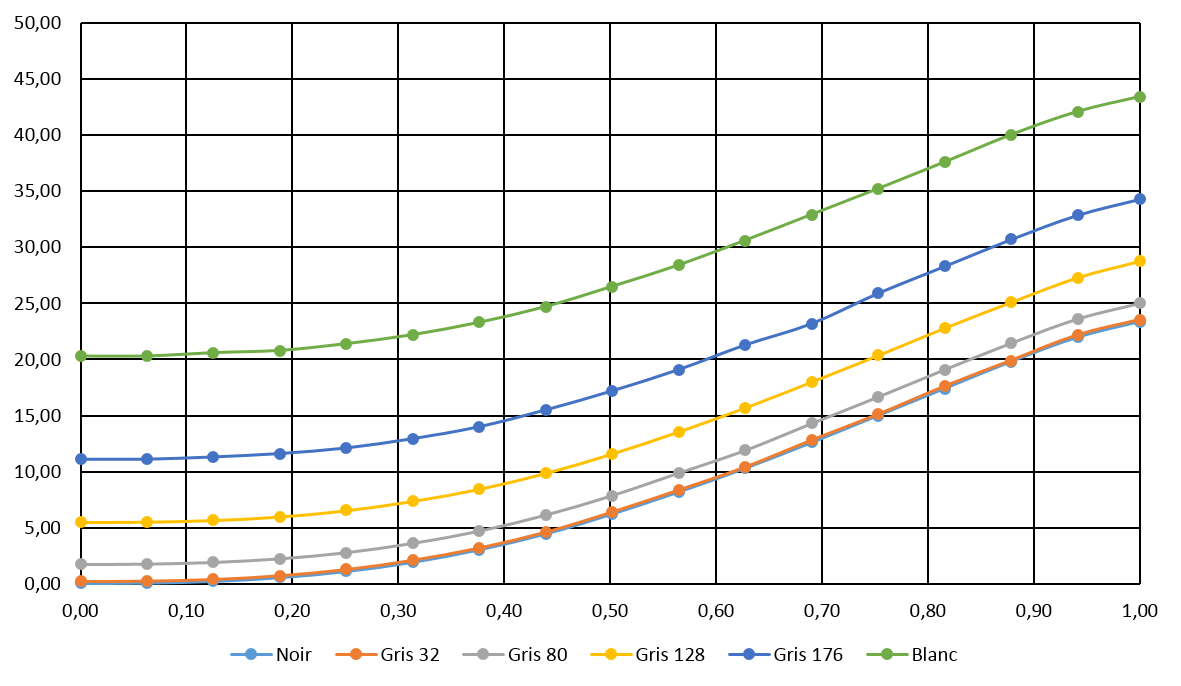
\includegraphics[scale=.75]{Figures/EvolutionLuminanceTarget}
		\caption{Luminance de la cible en fonction de la luminance globale}
		\label{fig:evolution_luminance_target}
	\end{figure}
	
	\section{Diamètre pupillaire}
	\par L'objectif était de vérifier une hypothèse: la luminance mesurée sur les écrans est égale à la luminance d'adaptation. Pour ce faire, toutes les mesures précédentes ont été faites par une personne équipée d'un oculomètre commercialisé par la société Ergoneers, le Dikablis Profressional\footnote{\url{https://lc.cx/dgLn}} (Fig. \ref{fig:dikablis_pro}). Si on arrive à récupérer le diamètre pupillaire réel, mesuré en temps réel sur l'opérateur des mesures, on pourra, via la littérature et notamment la formule de Weale (Eq. \ref{eq:weale_equation}) remonter à la luminance d'adaptation qui provoque ce diamètre pupillaire. On pourra alors la comparer à la luminance mesurée sur nos écrans et discuter notre hypothèse.
	
	\begin{equation}
		2r = 4.77 - 2.44~\tanh[0.3~\log_{10}(L_a)]
		\label{eq:weale_equation}
	\end{equation}
	
	\begin{figure}
		\centering
		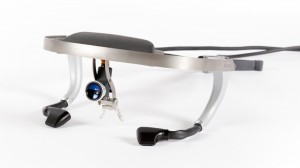
\includegraphics[scale=1]{Figures/DikablisProfessional}
		\caption{Oculomètre Dikablis Professional}
		\label{fig:dikablis_pro}
	\end{figure}
	
	\par L'oculomètre filme les yeux dans le cadre de son fonctionnement et permet donc de relever parallèlement un certain nombre d'autres paramètres en temps réel et sur les deux yeux indépendamment. Notamment, la surface, la hauteur et la largeur pupillaire peuvent être mesurées. La Fig. \ref{fig:mesure_pupille} représente une mesure de largeur pupillaire au cours du temps. Les pics correspondent à un clignement des yeux. Malheureusement, ces mesures sont données en pixels et non pas directement en mm. Il faut donc faire une conversion par rapport à une référence connue (en millimètres) dans l'image.
	
	\begin{figure}
		\centering
		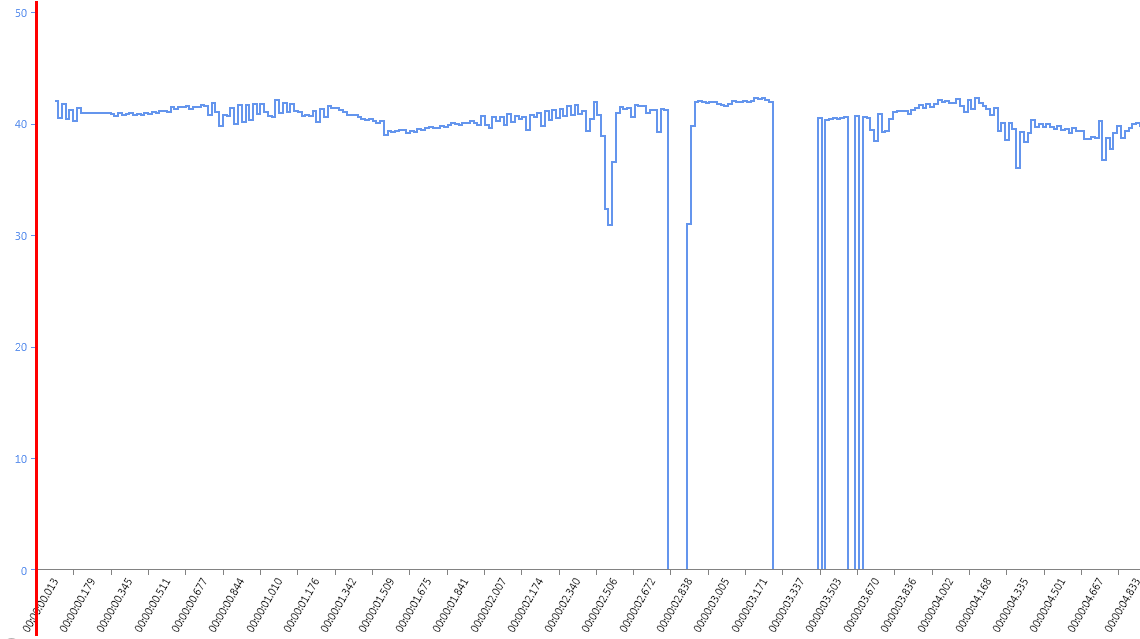
\includegraphics[scale=.5]{Figures/LargeurPupillaireEnFonctionDuTemps}
		\caption{Exemple d'une mesure en pixel de largeur pupillaire au cours du temps.}
		\label{fig:mesure_pupille}
	\end{figure}
	
	\par On prend le diamètre du globe oculaire comme référence car sa taille est globalement constante (Fig. \ref{fig:mesure_reference}). Sur l'opérateur des mesures, cette valeur était de $25~mm$. En mesurant ensuite directement sur une image, qu'on prend comme référence, la largeur de l'œil (mesure de référence) et le diamètre de la pupille on peut obtenir un ratio transformant une taille mesurée en pixel par le logiciel en millimètres réels (Eq. \ref{eq:ratio_mesure_eye_tracker}).
	
	\begin{equation}
		r = \frac{diam~oculaire~mesure~reelle~(mm) \times diam~pupillaire~image~ref~(mm)}{diam~oculaire~image~ref~(mm) \times diam~pupillaire~image~ref~(px)}
		\label{eq:ratio_mesure_eye_tracker}
	\end{equation}
	
	\par De même que précédemment, on prend des mesures	dans cinq conditions de luminosité: condition de luminosité maximale, condition minimale et trois conditions intermédiaires. Les mesures sont disponibles dans en Table \ref{tab:mesure_pupillaire} et sur la Fig. \ref{fig:resultats_mesure_pupille}.
	
	\begin{table}[h]	
		\centering
		\caption{Mesure pupillaires en fonction de la luminosité}
		\label{tab:mesure_pupillaire}
		\small
		\begin{tabular}{ccccc}
			\textbf{Gris} & \textbf{Luminance} & \textbf{Diam. théorique} & \textbf{Diam. mesuré œil gauche} & \textbf{Diam. mesuré œil droit}\\
			0 & $0.53~cd/m^2$ & $5.59~mm$ & $5.00~mm$ & $4.97~mm$\\
			64 & $2.09~cd/m^2$ & $4.54~mm$ & $3.75~mm$ & $3.21~mm$\\
			128 & $11.72~cd/m^2$ & $4.01~mm$ & $3.42~mm$ & $3.07~mm$\\
			192 & $27.62~cd/m^2$ & $3.78~mm$ & $2.70~mm$ & $2.53~mm$\\
			255 & $42.82~cd/m^2$ & $3.66~mm$ & $2.45~mm$ & $2.23~mm$\\
		\end{tabular}
	\end{table}
	
	\begin{figure}
		\centering
		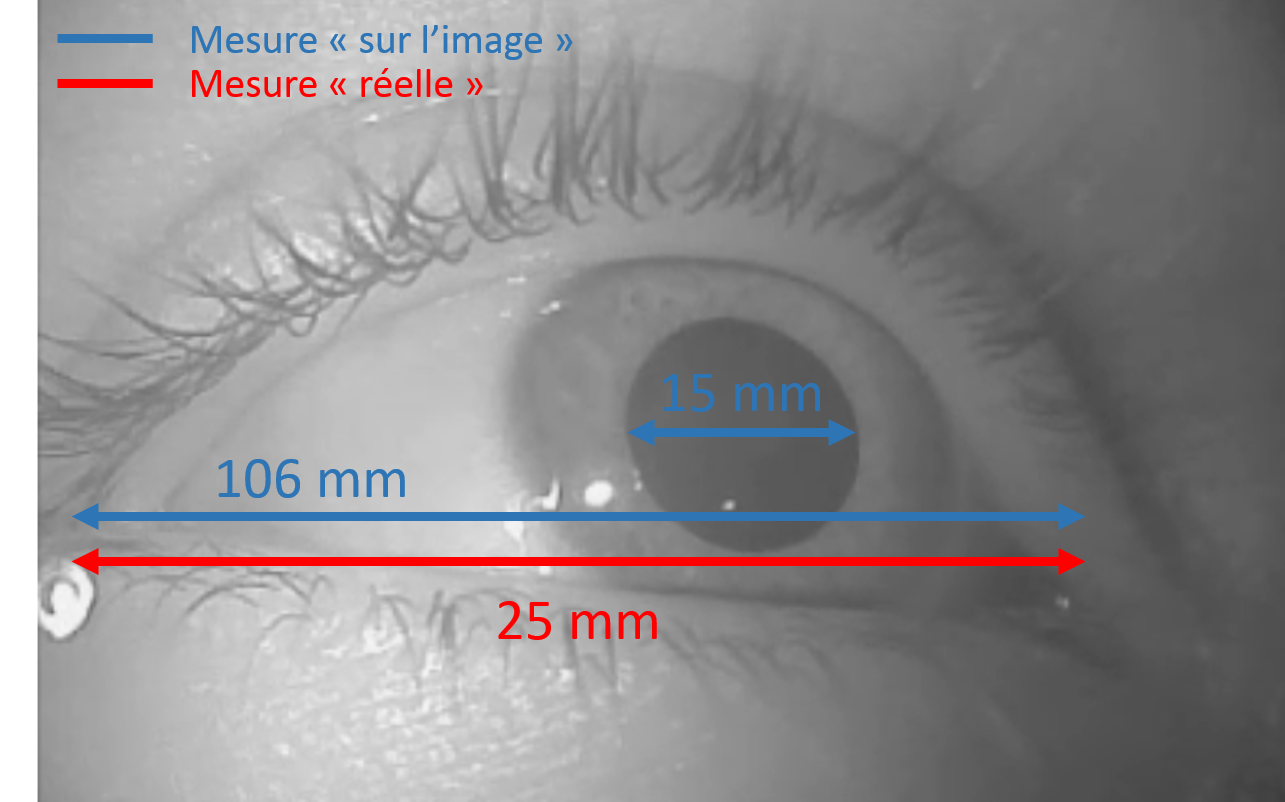
\includegraphics[scale=.7]{Figures/MesureReferenceOeil}
		\caption{Mesures pour la conversion pixel/mm.}
		\label{fig:mesure_reference}
	\end{figure}
	
	\par La mesure est très imprécise et souffre de plusieurs facteurs d'erreurs: d'une part la mesure logicielle en pixel sur laquelle on ne peut avoir aucun contrôle, d'autre part, les mesures <<~à la règle~>> de la mesure de référence sur l'oeil de l'opérateur et des valeurs sur l'image de référence pour le ratio sont assez imprécises et peuvent varier à l'ordre de grandeur du millimètre, ce qui est très important vis à vis des valeurs finales.
	
	\par Par conséquent nos mesures sont relativement éloignées des diamètres théoriques calculés en fonction de la luminance venant des écrans (Fig. \ref{fig:resultats_mesure_pupille}). Cela ne permet donc pas de valider, ni d'invalider, notre hypothèse de départ qui était l'égalité entre la luminance générée par les écrans et la luminance d'adaptation des yeux. L'expérimentation devra donc se faire en posant cette hypothèse.
	
	\begin{figure}
		\centering
		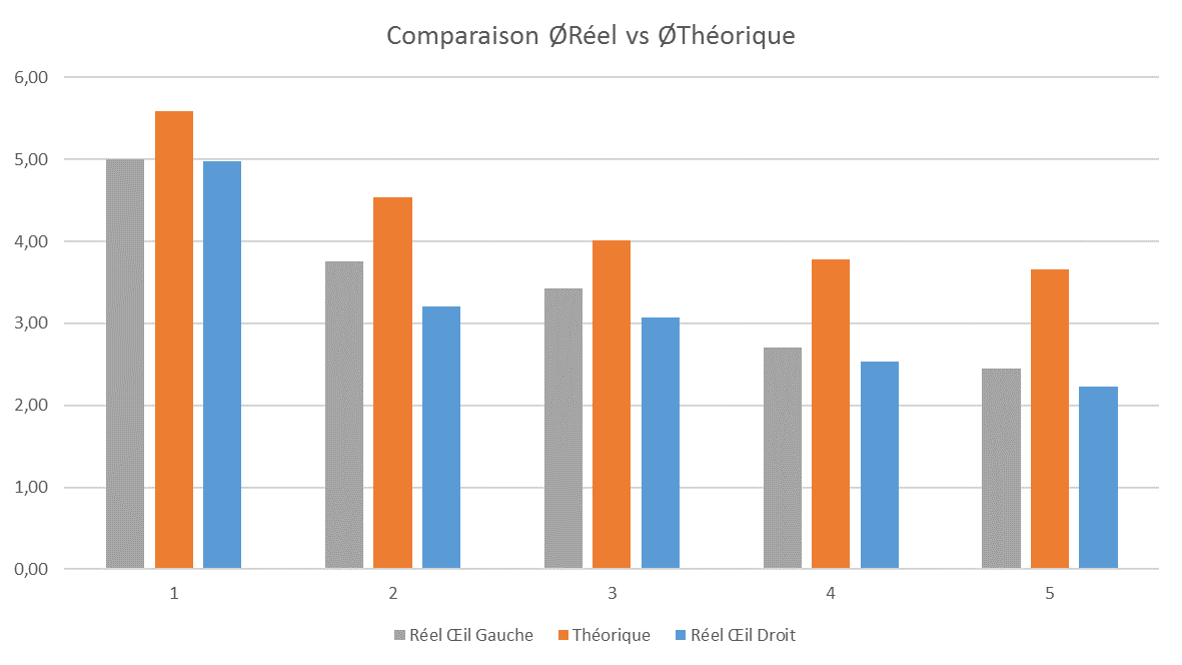
\includegraphics[scale=.75]{Figures/ComparaisonDiamReelDiamTheo}
		\caption{Comparaison entre les mesures de diamètre pupillaire par rapport aux valeurs théoriques fonction de la luminance affichée.}
		\label{fig:resultats_mesure_pupille}
	\end{figure}
	
	\section{Absorption des verres des lunettes 3D}
	\par On profite également de ces séries de mesures préliminaires pour vérifier un chiffre donné par le constructeur des lunettes: seulement 17\% de la luminosité globale arrive à l'œil après les lunettes stéréoscopiques. Cette donnée aurait pu nous servir directement en tant que valeur de transmittance $T$ si on avait voulu réaliser notre expérimentation en stéréoscopie. Même si on choisira par la suite de faire passer nos sujets en conditions monoscopiques, il reste intéressant de vérifier ce chiffre de 17\% avant sans justifications.
	
	\begin{figure}
		\centering
		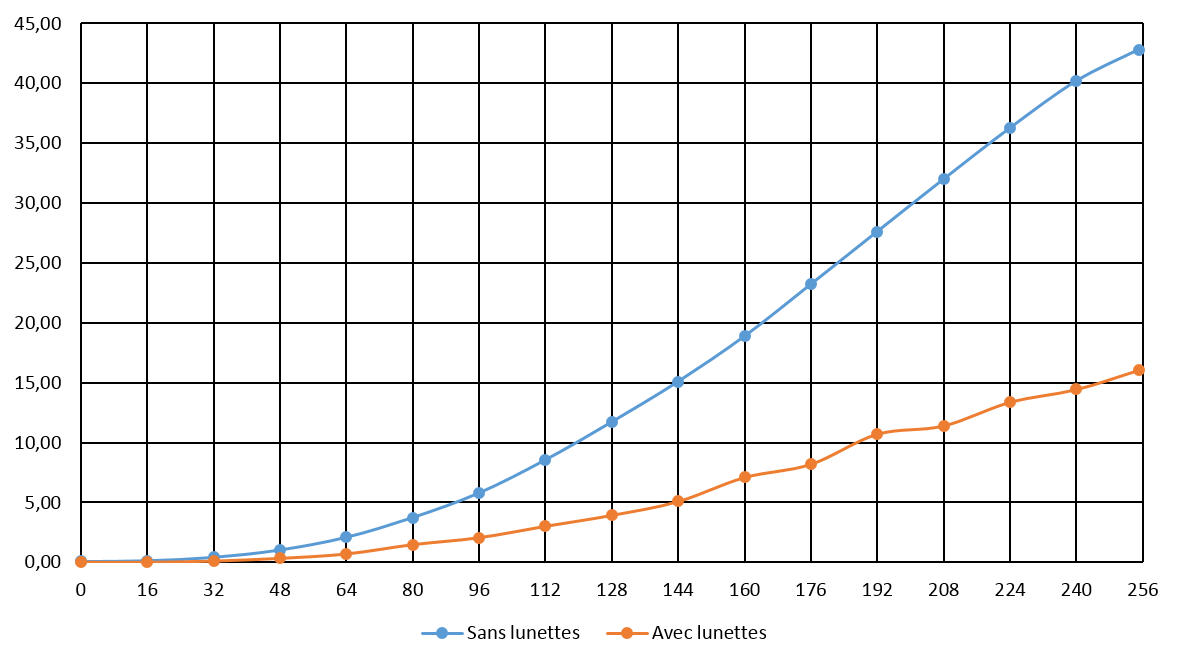
\includegraphics[scale=.75]{Figures/CourbesLuminanceLunettesStereo}
		\caption{Comparaison des mesures sans et avec filtre des lunettes stéréoscopiques.}
		\label{fig:pourcentage absorption}
	\end{figure}
	
	\par En parallèle des mesures décrites précédemment pour la luminance globale, on réalise également des mesures à travers un des deux verres de lunettes stéréoscopiques. Les résultats sont très probants (Fig. \ref{fig:pourcentage absorption}) et donnent une valeur d'absorption moyenne à 65\% sur toute la gamme de luminances possibles dans le simulateur soit un taux d'absorption de 35\%. Cependant, par construction, en stéréoscopie, les verres ne laissent passer la lumière que la moitié du temps pour permettre de nourrir chaque œil avec la bonne image. On retrouve donc bien la valeur de 17\% annoncée par le constructeur.
	
	\par Là encore, on déduit une régression polynomiale d'ordre 3 ($R^2 = 1$) qui nous donne la relation mathématique (Eq. \ref{eq:regression_luminance_filtre}) permettant d'anticiper la luminance reçue à travers les verres de lunettes stéréoscopiques en fonction du niveau de gris. Avec $L_F$ la luminance de la face avant du simulateur à travers le filtre et $g$ le niveau de gris normalisé.
	
	\begin{equation}
		L_C(g) = 0.26 - 6.82~g + 36.55~g^2 - 13.86~g^3
		\label{eq:regression_luminance_filtre}
	\end{equation}
	
	\begin{figure}
		\centering
		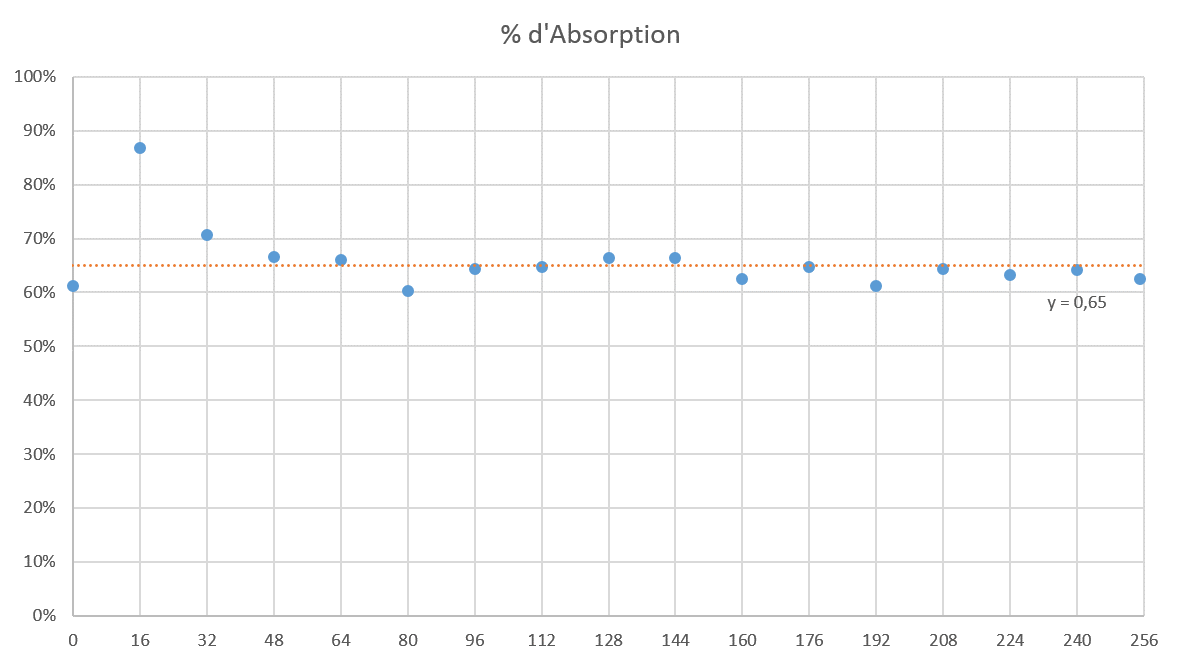
\includegraphics[scale=.75]{Figures/PourcentageAbsorption}
		\caption{Pourcentage d'absorption en fonction du niveau de gris affiché.}
		\label{fig:pourcentage absorption}
	\end{figure}
	
	\par On possède désormais tous les éléments pour se lancer dans la vérification expérimentale du modèle de Rea: on connait parfaitement le comportement en luminance du simulateur, on a vérifié le taux d'absorption des lunettes et on sait que l'hypothèse reliant la luminance de fond et la luminance d'adaptation doit être faite, faute d'avoir pu la démontrer quantitativement.
